% fancytikzposter.tex, version 2.1
% Original template created by Elena Botoeva [botoeva@inf.unibz.it], June 2012
%
% This file is distributed under the Creative Commons Attribution-NonCommercial 2.0
% Generic (CC BY-NC 2.0) license
% http://creativecommons.org/licenses/by-nc/2.0/


\documentclass{a0poster}

\usepackage{2018-ExcelFIT-MaestroPerformance-poster}



%%%%% --------- Change here if you want ---------- %%%%%
%% margin for the geometry package, must be changed before using the geometry package
%% default value is 4cm
\setmargin{2}

%% the space between the blocks
%% default value is 2cm
\setblockspacing{1}

%% the height of the title stripe in block nodes, decrease it to save space
%% default value is 3cm
\setblocktitleheight{3}

%% the number of columns in the poster, possible values 2,3
%% default value is 2
% \setcolumnnumber{3}

%% the space between two or more groups of authors from different institutions
%% used in \maketitle
% \setinstituteshift{10}

%% which template to use
%% N1 simple, standard look, with a colored background and gray boxes
%% N2 board with nodes
%% N3 another standard look
%% N4 envelope-like look
%% N5 with a wave-like head, original idea taken from
%%%% http://fc09.deviantart.net/fs71/f/2010/322/1/1/scientific_poster_by_nabuy-d333ria.jpg
\usetemplate{1}

%% components of the templates
%% (the maximal possible numbers are mentioned as the parameters)
% \usecolortemplate{4}
\usebackgroundtemplate{1}
% \usetitletemplate{2}
\useblocknodetemplate{4}
\useplainblocktemplate{4}
\useinnerblocktemplate{4}


%% the height of the head drawing on top
%% applicable to templates N3, 4 and 5
% \setheaddrawingheight{14}


%% change the basic colors
\definecolor{myblue}{HTML}{B5D7ED}
\definecolor{mygreen}{HTML}{C5E3DF}
%\setfirstcolor{myblue}% default 116699
%\setsecondcolor{gray!80!}% default CCCCCC
%\setthirdcolor{red!80!black}% default 991111

%% change the more specific colors
% \setbackgrounddarkcolor{colorone!70!black}
% \setbackgroundlightcolor{colorone!70!}
% \settitletextcolor{textcolor}
% \settitlefillcolor{white}
% \settitledrawcolor{myblue}
% \setblocktextcolor{textcolor}
% \setblockfillcolor{white}
% \setblocktitletextcolor{colorone}
% \setblocktitlefillcolor{colortwo} %the color of the border
% \setplainblocktextcolor{textcolor}
% \setplainblockfillcolor{colorthree!40!}
% \setplainblocktitletextcolor{textcolor}
% \setplainblocktitlefillcolor{colorthree!60!}
% \setinnerblocktextcolor{textcolor}
% \setinnerblockfillcolor{white}
% \setinnerblocktitletextcolor{white}
% \setinnerblocktitlefillcolor{colorthree}

%% Color changes
% Title bar color
\settitledrawcolor{myblue}
% Block title color
\setblocktitletextcolor{black}
% Block fill collor
\setblocktitlefillcolor{myblue}


%%% size of the document and the margins
%% A0
% \usepackage[margin=\margin cm, paperwidth=118.9cm, paperheight=84.1cm]{geometry}
% \usepackage[margin=\margin cm, paperwidth=84.1cm, paperheight=118.9cm]{geometry}
%% A1
\usepackage[margin=\margin cm, paperwidth=59.4cm, paperheight=84.1cm]{geometry}
%% B1
% \usepackage[margin=\margin cm, paperwidth=70cm, paperheight=100cm]{geometry}



%% changing the fonts
\usepackage{cmbright}
%\usepackage[default]{cantarell}
%\usepackage{avant}
%\usepackage[math]{iwona}
\usepackage[math]{kurier}
% \usepackage[T1]{fontenc}
\usepackage{times}


%% add your packages here
\usepackage{hyperref}





\title{Performance testing and analysis of Qpid-dispatch router}
\author{Jakub Stejskal\\
  Faculty of Technology, Brno University of Technology\\
  \texttt{xstejs24@stud.fit.vutbr.cz}\\
  \textbf{32}
}


\begin{document}



%%%%% ---------- the background picture ---------- %%%%%
%% to change it modify the macro \BackgroundPicture
\ClearShipoutPicture
\AddToShipoutPicture{\BackgroundPicture}

\noindent % to have the picture right in the center
\begin{tikzpicture}
  \initializesizeandshifts
  % \setxshift{15}
  % \setyshift{2}


  %% the title block, #1 - shift, the default value is (0,0), #2 - width, #3 - scale
  %% the alias of the title block is `title', so we can refer to its boundaries later
  \ifthenelse{\equal{\template}{1}}{
    \titleblock{67}{0.8}
  }{
    \titleblock{67}{1}
  }

  %% a logo can be added to the title block
  %% #1 - anchor relative to the title block, #2 - shift, #3 - width, #3 - file name
  \addlogo[south west]{(2,1)}{10cm}{ExcelAtFIT-logo.pdf}
  \addlogo[south east]{(-2,1)}{3cm}{maestro-logo.pdf}
  \addlogo[south east]{(-6,0.2)}{7cm}{redhat-vector-logo.png}

  %% a block node, with the specified position (optional), title and the content
  %% #1 - where (optional), #2 - title, #3 - text
  %%%%%%%%%% ------------------------------------------ %%%%%%%%%%
  \blocknode%
  {Messaging Performance Tool}%
  {
      \emph{Messaging Performance Tool \textbf{(Maestro)}} is a testing system designed for testing the performance of \textbf{Message Oriented Middleware} (MOM)

      \begin{tikzfigure}[Scheme of communication and protocols used between the Messaging Performance Tool and testing nodes.]
          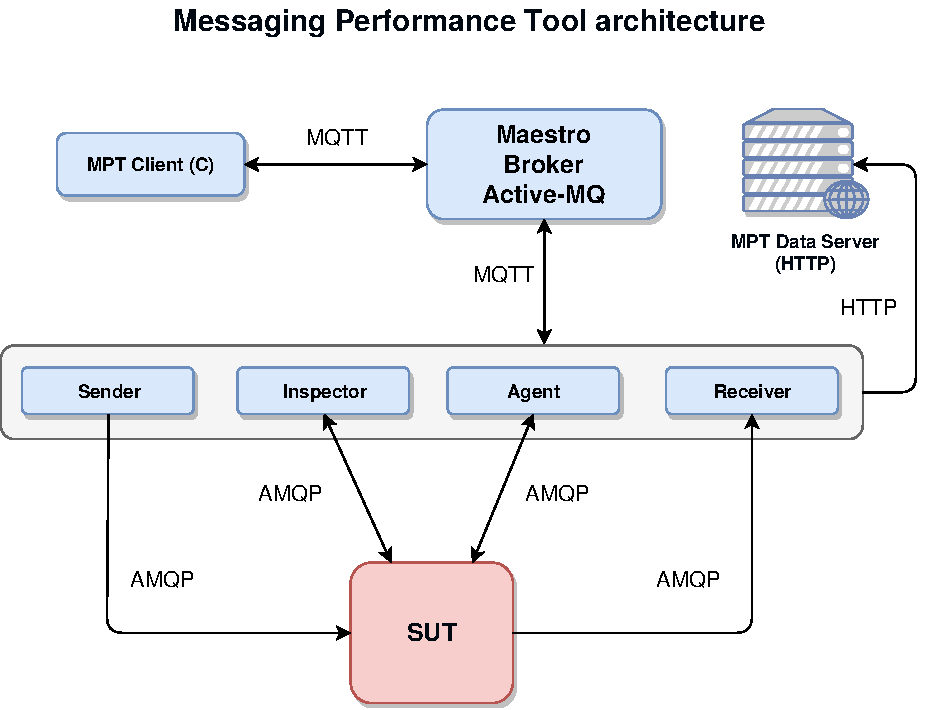
\includegraphics[width=0.7\linewidth]{figures/msg_perf_tool.pdf}
      \end{tikzfigure}

      Maestro is able to monitor each testing node and collect data to help improve the performance. Maestro is focused on performance testing of \textbf{Messaging Broker}. For expand the capabilities of Maestro to perform behavioral testing we need new extension module.
  }


  %% by default, the position of the new block node is right below the previous
  %% block node, stored in (currenty)
  %% box is the alias of the previous block, so we can refer to its boundaries

  %%%%%%%%%% ------------------------------------------ %%%%%%%%%%
  \blocknode{Topology Generator}%
  {
    For automatic deployment and node configuration we use \textbf{Ansible} and \textbf{Topology Generator}. We are able to generate configuration files and deploy them via one simple YAML script.
    \begin{tikzfigure}[Example of router topology generation and deployment.]
        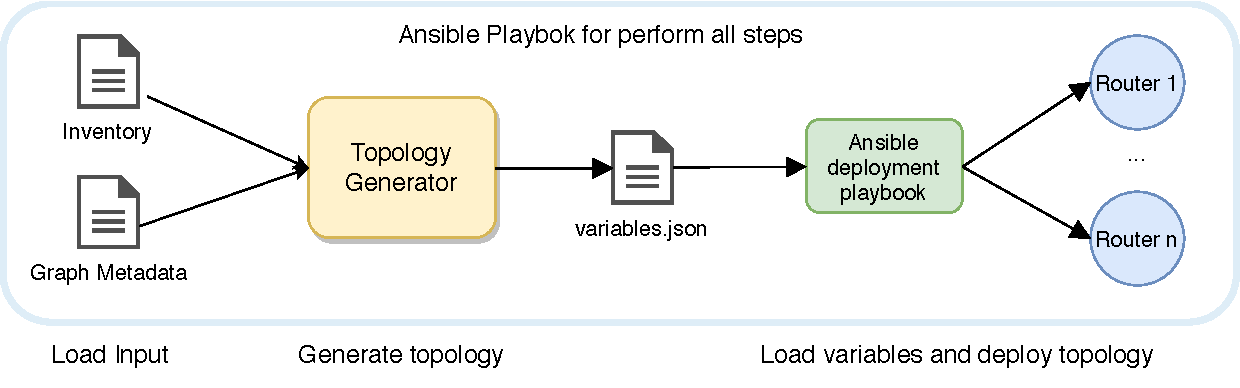
\includegraphics[width=0.9\linewidth]{figures/generator_poster.pdf}
    \end{tikzfigure}
  }


  \blocknode{Throughput Measurements}%
  {
    Maestro is able to compute \textbf{throughput} of \textbf{single node} or whole topology consisting of \textbf{multiple nodes}.
    \begin{tikzfigure}[Chart of maximum throughput of router service and broker service during specific test cases with specific node configuration.]
        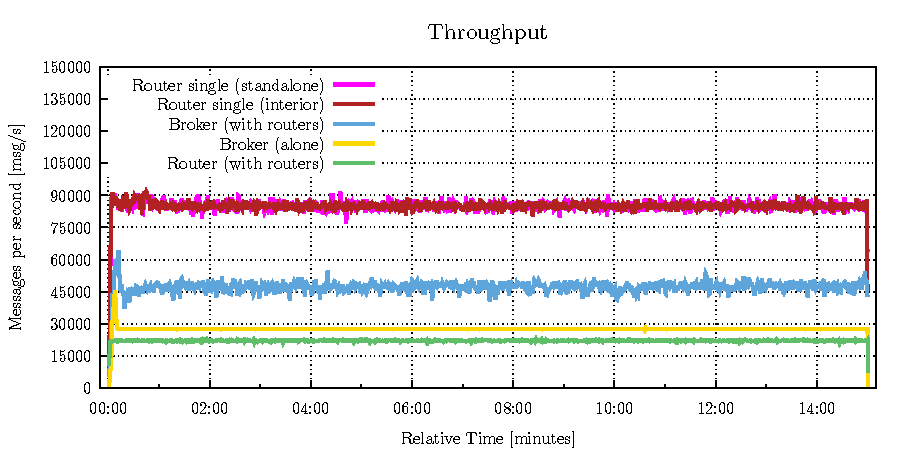
\includegraphics[width=1\linewidth]{figures/throughput.pdf}
    \end{tikzfigure}
  }

  %%%%%%%%%%%%% NEW COLUMN %%%%%%%%%%%%%%%
  \startsecondcolumn

  %%%%%%%%%% ------------------------------------------ %%%%%%%%%%
  \blocknode%
  {Maestro Extensions}%
  {
    \textbf{Maestro Agent}
    \begin{itemize}
      \item Behavioral performance testing
      \item Execute user specified code from git repository on each test node by Groovy
    \end{itemize}

    \begin{tikzfigure}[A shaded circle]
        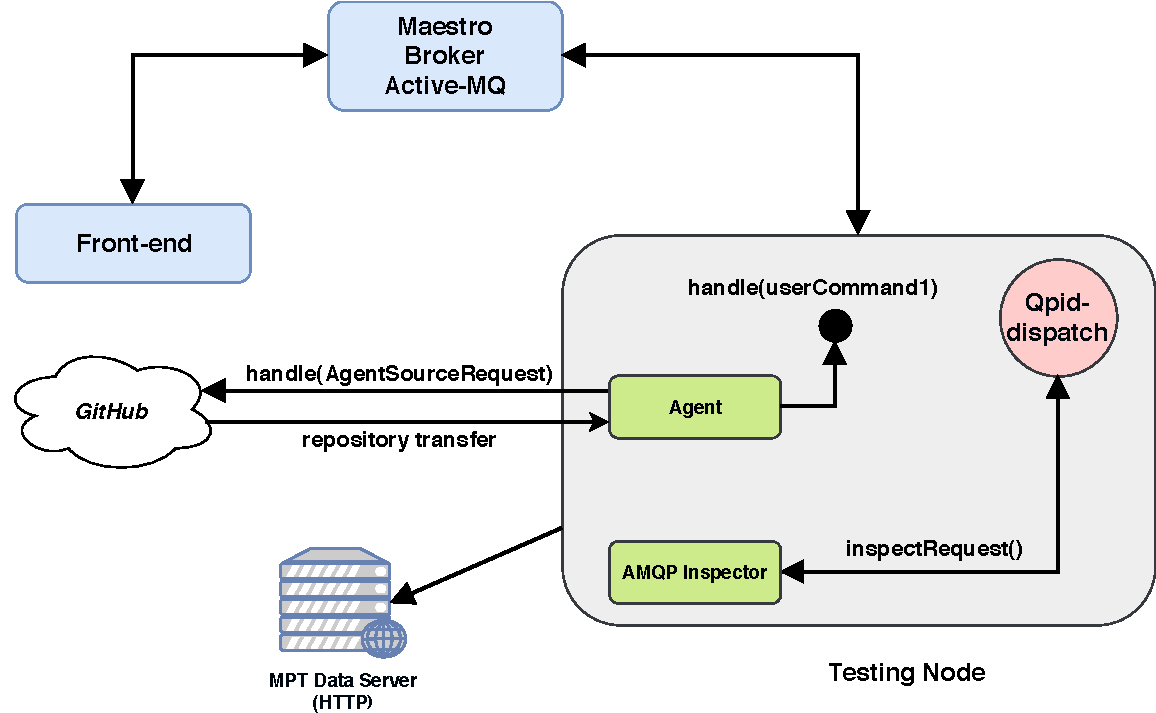
\includegraphics[width=0.8\linewidth]{figures/agent_demo.pdf}
    \end{tikzfigure}

    \textbf{Maestro AMQP Inspector}
    \begin{itemize}
      \item Monitor inner informations about Qpid-dispatch router
      \item Collect and report data to data server
    \end{itemize}
  }



  %%%%%%%%%% ------------------------------------------ %%%%%%%%%%
  \blocknode{Latency Measurements}%
  {
    Maestro is able to measure \textbf{latency} on over the topology. Latency is measured between message send time and receive time.
    \begin{tikzfigure}[Latency chart showing the difference between router service and broker service latency at 80\,\% of maximum rate.]
        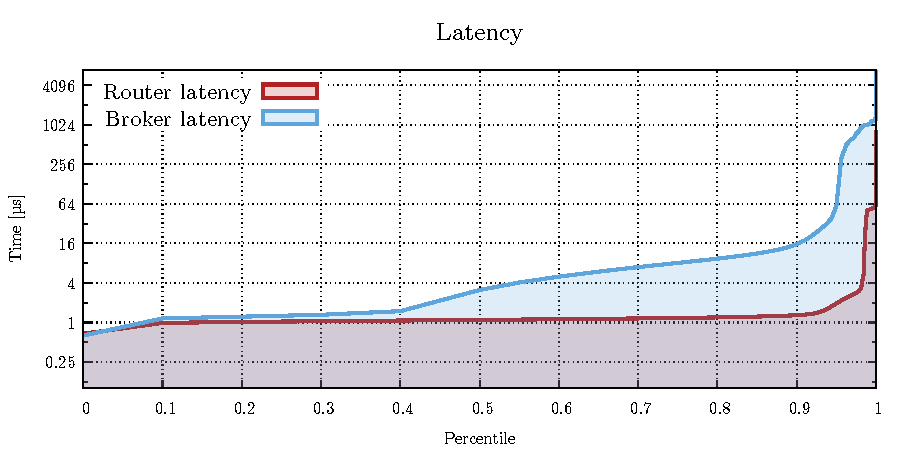
\includegraphics[width=0.90\linewidth]{figures/latency.pdf}
    \end{tikzfigure}

    The agent can influence performance with his action such as shut down one node, change the router configuration or change setting of network interface. All these actions can influence the latency and message delivery time.
    \begin{tikzfigure}[Latency chart showing the results of tests with agent actions. The agent shut down one of the test node during the test.]
        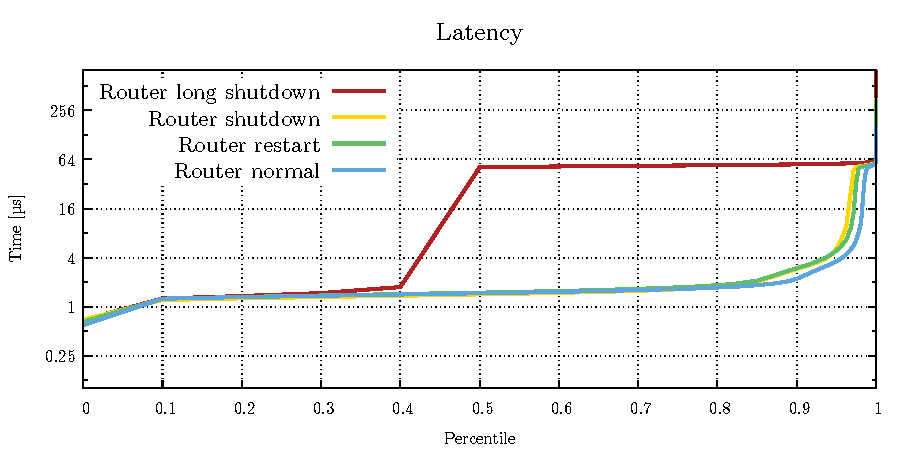
\includegraphics[width=0.90\linewidth]{figures/agent_latency.pdf}
    \end{tikzfigure}
  }

\end{tikzpicture}


\end{document}
